% Options for packages loaded elsewhere
\PassOptionsToPackage{unicode}{hyperref}
\PassOptionsToPackage{hyphens}{url}
%
\documentclass[
]{article}
\usepackage{amsmath,amssymb}
\usepackage{iftex}
\ifPDFTeX
  \usepackage[T1]{fontenc}
  \usepackage[utf8]{inputenc}
  \usepackage{textcomp} % provide euro and other symbols
\else % if luatex or xetex
  \usepackage{unicode-math} % this also loads fontspec
  \defaultfontfeatures{Scale=MatchLowercase}
  \defaultfontfeatures[\rmfamily]{Ligatures=TeX,Scale=1}
\fi
\usepackage{lmodern}
\ifPDFTeX\else
  % xetex/luatex font selection
\fi
% Use upquote if available, for straight quotes in verbatim environments
\IfFileExists{upquote.sty}{\usepackage{upquote}}{}
\IfFileExists{microtype.sty}{% use microtype if available
  \usepackage[]{microtype}
  \UseMicrotypeSet[protrusion]{basicmath} % disable protrusion for tt fonts
}{}
\makeatletter
\@ifundefined{KOMAClassName}{% if non-KOMA class
  \IfFileExists{parskip.sty}{%
    \usepackage{parskip}
  }{% else
    \setlength{\parindent}{0pt}
    \setlength{\parskip}{6pt plus 2pt minus 1pt}}
}{% if KOMA class
  \KOMAoptions{parskip=half}}
\makeatother
\usepackage{xcolor}
\usepackage[margin=1in]{geometry}
\usepackage{color}
\usepackage{fancyvrb}
\newcommand{\VerbBar}{|}
\newcommand{\VERB}{\Verb[commandchars=\\\{\}]}
\DefineVerbatimEnvironment{Highlighting}{Verbatim}{commandchars=\\\{\}}
% Add ',fontsize=\small' for more characters per line
\usepackage{framed}
\definecolor{shadecolor}{RGB}{248,248,248}
\newenvironment{Shaded}{\begin{snugshade}}{\end{snugshade}}
\newcommand{\AlertTok}[1]{\textcolor[rgb]{0.94,0.16,0.16}{#1}}
\newcommand{\AnnotationTok}[1]{\textcolor[rgb]{0.56,0.35,0.01}{\textbf{\textit{#1}}}}
\newcommand{\AttributeTok}[1]{\textcolor[rgb]{0.13,0.29,0.53}{#1}}
\newcommand{\BaseNTok}[1]{\textcolor[rgb]{0.00,0.00,0.81}{#1}}
\newcommand{\BuiltInTok}[1]{#1}
\newcommand{\CharTok}[1]{\textcolor[rgb]{0.31,0.60,0.02}{#1}}
\newcommand{\CommentTok}[1]{\textcolor[rgb]{0.56,0.35,0.01}{\textit{#1}}}
\newcommand{\CommentVarTok}[1]{\textcolor[rgb]{0.56,0.35,0.01}{\textbf{\textit{#1}}}}
\newcommand{\ConstantTok}[1]{\textcolor[rgb]{0.56,0.35,0.01}{#1}}
\newcommand{\ControlFlowTok}[1]{\textcolor[rgb]{0.13,0.29,0.53}{\textbf{#1}}}
\newcommand{\DataTypeTok}[1]{\textcolor[rgb]{0.13,0.29,0.53}{#1}}
\newcommand{\DecValTok}[1]{\textcolor[rgb]{0.00,0.00,0.81}{#1}}
\newcommand{\DocumentationTok}[1]{\textcolor[rgb]{0.56,0.35,0.01}{\textbf{\textit{#1}}}}
\newcommand{\ErrorTok}[1]{\textcolor[rgb]{0.64,0.00,0.00}{\textbf{#1}}}
\newcommand{\ExtensionTok}[1]{#1}
\newcommand{\FloatTok}[1]{\textcolor[rgb]{0.00,0.00,0.81}{#1}}
\newcommand{\FunctionTok}[1]{\textcolor[rgb]{0.13,0.29,0.53}{\textbf{#1}}}
\newcommand{\ImportTok}[1]{#1}
\newcommand{\InformationTok}[1]{\textcolor[rgb]{0.56,0.35,0.01}{\textbf{\textit{#1}}}}
\newcommand{\KeywordTok}[1]{\textcolor[rgb]{0.13,0.29,0.53}{\textbf{#1}}}
\newcommand{\NormalTok}[1]{#1}
\newcommand{\OperatorTok}[1]{\textcolor[rgb]{0.81,0.36,0.00}{\textbf{#1}}}
\newcommand{\OtherTok}[1]{\textcolor[rgb]{0.56,0.35,0.01}{#1}}
\newcommand{\PreprocessorTok}[1]{\textcolor[rgb]{0.56,0.35,0.01}{\textit{#1}}}
\newcommand{\RegionMarkerTok}[1]{#1}
\newcommand{\SpecialCharTok}[1]{\textcolor[rgb]{0.81,0.36,0.00}{\textbf{#1}}}
\newcommand{\SpecialStringTok}[1]{\textcolor[rgb]{0.31,0.60,0.02}{#1}}
\newcommand{\StringTok}[1]{\textcolor[rgb]{0.31,0.60,0.02}{#1}}
\newcommand{\VariableTok}[1]{\textcolor[rgb]{0.00,0.00,0.00}{#1}}
\newcommand{\VerbatimStringTok}[1]{\textcolor[rgb]{0.31,0.60,0.02}{#1}}
\newcommand{\WarningTok}[1]{\textcolor[rgb]{0.56,0.35,0.01}{\textbf{\textit{#1}}}}
\usepackage{graphicx}
\makeatletter
\def\maxwidth{\ifdim\Gin@nat@width>\linewidth\linewidth\else\Gin@nat@width\fi}
\def\maxheight{\ifdim\Gin@nat@height>\textheight\textheight\else\Gin@nat@height\fi}
\makeatother
% Scale images if necessary, so that they will not overflow the page
% margins by default, and it is still possible to overwrite the defaults
% using explicit options in \includegraphics[width, height, ...]{}
\setkeys{Gin}{width=\maxwidth,height=\maxheight,keepaspectratio}
% Set default figure placement to htbp
\makeatletter
\def\fps@figure{htbp}
\makeatother
\setlength{\emergencystretch}{3em} % prevent overfull lines
\providecommand{\tightlist}{%
  \setlength{\itemsep}{0pt}\setlength{\parskip}{0pt}}
\setcounter{secnumdepth}{-\maxdimen} % remove section numbering
\ifLuaTeX
  \usepackage{selnolig}  % disable illegal ligatures
\fi
\IfFileExists{bookmark.sty}{\usepackage{bookmark}}{\usepackage{hyperref}}
\IfFileExists{xurl.sty}{\usepackage{xurl}}{} % add URL line breaks if available
\urlstyle{same}
\hypersetup{
  pdftitle={Question 6},
  hidelinks,
  pdfcreator={LaTeX via pandoc}}

\title{Question 6}
\author{}
\date{\vspace{-2.5em}2023-12-01}

\begin{document}
\maketitle

\hypertarget{r-markdown}{%
\subsection{R Markdown}\label{r-markdown}}

This is an R Markdown document. Markdown is a simple formatting syntax
for authoring HTML, PDF, and MS Word documents. For more details on
using R Markdown see \url{http://rmarkdown.rstudio.com}.

When you click the \textbf{Knit} button a document will be generated
that includes both content as well as the output of any embedded R code
chunks within the document. You can embed an R code chunk like this:

\begin{Shaded}
\begin{Highlighting}[]
\NormalTok{anov2}\OtherTok{=} \FunctionTok{lm}\NormalTok{(ges\_teqco2 }\SpecialCharTok{\textasciitilde{}}\NormalTok{TypeEPCI }\SpecialCharTok{*}\NormalTok{ annee\_inv, }\AttributeTok{data=}\NormalTok{dlog)}
\end{Highlighting}
\end{Shaded}

\hypertarget{moduxe8le-linuxe9aire}{%
\subsection{Modèle linéaire}\label{moduxe8le-linuxe9aire}}

Nous avons vu précédemment comment classer les données, de façon
supervisée ou non. Nous allons maintenant voir comment nous pouvons
expliquer les données. Nous allons effectuer différents modèles
linéaires, afin d'évaluer les variables expliquant : le gaz à effet de
serre, et l'

\begin{Shaded}
\begin{Highlighting}[]
\NormalTok{anov\_sans\_int}\OtherTok{=}\FunctionTok{lm}\NormalTok{(ges\_teqco2 }\SpecialCharTok{\textasciitilde{}}\NormalTok{TypeEPCI }\SpecialCharTok{+}\NormalTok{ annee\_inv, }\AttributeTok{data=}\NormalTok{dlog)}
\FunctionTok{anova}\NormalTok{(anov\_sans\_int,anov2)}
\end{Highlighting}
\end{Shaded}

\begin{verbatim}
## Analysis of Variance Table
## 
## Model 1: ges_teqco2 ~ TypeEPCI + annee_inv
## Model 2: ges_teqco2 ~ TypeEPCI * annee_inv
##   Res.Df    RSS Df Sum of Sq      F Pr(>F)
## 1    979 570.31                           
## 2    976 570.30  3 0.0085333 0.0049 0.9995
\end{verbatim}

\begin{Shaded}
\begin{Highlighting}[]
\NormalTok{anov\_annee}\OtherTok{=}\FunctionTok{lm}\NormalTok{(ges\_teqco2 }\SpecialCharTok{\textasciitilde{}}\NormalTok{annee\_inv, }\AttributeTok{data=}\NormalTok{dlog)}
\NormalTok{anov\_type}\OtherTok{=}\FunctionTok{lm}\NormalTok{(ges\_teqco2 }\SpecialCharTok{\textasciitilde{}}\NormalTok{TypeEPCI, }\AttributeTok{data=}\NormalTok{dlog)}

\FunctionTok{anova}\NormalTok{(anov\_annee,anov\_sans\_int)}
\end{Highlighting}
\end{Shaded}

\begin{verbatim}
## Analysis of Variance Table
## 
## Model 1: ges_teqco2 ~ annee_inv
## Model 2: ges_teqco2 ~ TypeEPCI + annee_inv
##   Res.Df    RSS Df Sum of Sq      F    Pr(>F)    
## 1    982 982.84                                  
## 2    979 570.31  3    412.53 236.05 < 2.2e-16 ***
## ---
## Signif. codes:  0 '***' 0.001 '**' 0.01 '*' 0.05 '.' 0.1 ' ' 1
\end{verbatim}

\begin{Shaded}
\begin{Highlighting}[]
\FunctionTok{anova}\NormalTok{(anov\_type,anov\_sans\_int)}
\end{Highlighting}
\end{Shaded}

\begin{verbatim}
## Analysis of Variance Table
## 
## Model 1: ges_teqco2 ~ TypeEPCI
## Model 2: ges_teqco2 ~ TypeEPCI + annee_inv
##   Res.Df    RSS Df Sum of Sq      F Pr(>F)
## 1    980 570.47                           
## 2    979 570.31  1   0.16143 0.2771 0.5987
\end{verbatim}

\begin{Shaded}
\begin{Highlighting}[]
\FunctionTok{anova}\NormalTok{(}\FunctionTok{lm}\NormalTok{(ges\_teqco2 }\SpecialCharTok{\textasciitilde{}}\DecValTok{1}\NormalTok{, }\AttributeTok{data=}\NormalTok{dlog),anov\_type)}
\end{Highlighting}
\end{Shaded}

\begin{verbatim}
## Analysis of Variance Table
## 
## Model 1: ges_teqco2 ~ 1
## Model 2: ges_teqco2 ~ TypeEPCI
##   Res.Df    RSS Df Sum of Sq      F    Pr(>F)    
## 1    983 983.00                                  
## 2    980 570.47  3    412.53 236.23 < 2.2e-16 ***
## ---
## Signif. codes:  0 '***' 0.001 '**' 0.01 '*' 0.05 '.' 0.1 ' ' 1
\end{verbatim}

\begin{Shaded}
\begin{Highlighting}[]
\FunctionTok{anova}\NormalTok{(anov\_type,anov2)}
\end{Highlighting}
\end{Shaded}

\begin{verbatim}
## Analysis of Variance Table
## 
## Model 1: ges_teqco2 ~ TypeEPCI
## Model 2: ges_teqco2 ~ TypeEPCI * annee_inv
##   Res.Df    RSS Df Sum of Sq      F Pr(>F)
## 1    980 570.47                           
## 2    976 570.30  4   0.16996 0.0727 0.9904
\end{verbatim}

On garde le modèle anov\_type:

\begin{Shaded}
\begin{Highlighting}[]
\FunctionTok{summary}\NormalTok{(anov\_type)}
\end{Highlighting}
\end{Shaded}

\begin{verbatim}
## 
## Call:
## lm(formula = ges_teqco2 ~ TypeEPCI, data = dlog)
## 
## Residuals:
##     Min      1Q  Median      3Q     Max 
## -4.2233 -0.4145 -0.0369  0.3839  2.8504 
## 
## Coefficients:
##                   Estimate Std. Error t value Pr(>|t|)    
## (Intercept)        1.28521    0.06797  18.909  < 2e-16 ***
## TypeEPCICC        -1.53937    0.07289 -21.119  < 2e-16 ***
## TypeEPCICU         1.05473    0.31881   3.308 0.000973 ***
## TypeEPCIMetropole  1.84123    0.23050   7.988 3.83e-15 ***
## ---
## Signif. codes:  0 '***' 0.001 '**' 0.01 '*' 0.05 '.' 0.1 ' ' 1
## 
## Residual standard error: 0.763 on 980 degrees of freedom
## Multiple R-squared:  0.4197, Adjusted R-squared:  0.4179 
## F-statistic: 236.2 on 3 and 980 DF,  p-value: < 2.2e-16
\end{verbatim}

On peut pas annuler 1 des paramètres, on ne peut donc pas regrouper des
modalités entre elles, et on garde donc ce modèle. On essaye de voir sa
capacité de prédiction:

\begin{Shaded}
\begin{Highlighting}[]
\NormalTok{dlog}\OtherTok{=}\NormalTok{data[}\DecValTok{4}\SpecialCharTok{:}\DecValTok{15}\NormalTok{]}
\NormalTok{data\_quant}\OtherTok{=}\NormalTok{data[}\DecValTok{4}\SpecialCharTok{:}\DecValTok{14}\NormalTok{]}
\NormalTok{data\_quant}\OtherTok{=}\FunctionTok{scale}\NormalTok{(}\FunctionTok{log}\NormalTok{(data\_quant))}
\NormalTok{dlog[}\DecValTok{1}\SpecialCharTok{:}\DecValTok{11}\NormalTok{]}\OtherTok{=}\NormalTok{data\_quant}
\NormalTok{dlog}\OtherTok{=}\FunctionTok{data.frame}\NormalTok{(dlog,}\AttributeTok{annee\_inv=}\NormalTok{data}\SpecialCharTok{$}\NormalTok{annee\_inv)}
\NormalTok{taille\_train}\OtherTok{=}\FunctionTok{round}\NormalTok{(}\FloatTok{0.7}\SpecialCharTok{*}\FunctionTok{nrow}\NormalTok{(dlog))}
\NormalTok{d\_train}\OtherTok{=}\NormalTok{dlog[}\DecValTok{1}\SpecialCharTok{:}\NormalTok{taille\_train,]}
\NormalTok{d\_test}\OtherTok{=}\NormalTok{dlog[taille\_train}\SpecialCharTok{:}\FunctionTok{nrow}\NormalTok{(dlog),]}

\NormalTok{mod\_anov}\OtherTok{=}\FunctionTok{lm}\NormalTok{(ges\_teqco2 }\SpecialCharTok{\textasciitilde{}}\NormalTok{TypeEPCI, }\AttributeTok{data=}\NormalTok{d\_train)}
\NormalTok{pred}\OtherTok{=}\FunctionTok{predict}\NormalTok{(mod\_anov,d\_test)}
\NormalTok{resultat}\OtherTok{=}\FunctionTok{data.frame}\NormalTok{(}\AttributeTok{vrai\_ges=}\NormalTok{d\_test}\SpecialCharTok{$}\NormalTok{ges\_teqco2,}\AttributeTok{prediction=}\NormalTok{pred,}\AttributeTok{ecart=}\FunctionTok{abs}\NormalTok{(d\_test}\SpecialCharTok{$}\NormalTok{ges\_teqco2}\SpecialCharTok{{-}}\NormalTok{pred),}\AttributeTok{erreur\_pourcentage=}\FunctionTok{abs}\NormalTok{(d\_test}\SpecialCharTok{$}\NormalTok{ges\_teqco2}\SpecialCharTok{{-}}\NormalTok{pred)}\SpecialCharTok{/}\FunctionTok{abs}\NormalTok{(d\_test}\SpecialCharTok{$}\NormalTok{ges\_teqco2))}
\FunctionTok{summary}\NormalTok{(resultat)}
\end{Highlighting}
\end{Shaded}

\begin{verbatim}
##     vrai_ges           prediction           ecart          erreur_pourcentage 
##  Min.   :-4.452839   Min.   :-0.25492   Min.   :0.001541   Min.   :   0.0060  
##  1st Qu.:-0.609488   1st Qu.:-0.25492   1st Qu.:0.192698   1st Qu.:   0.4282  
##  Median :-0.114984   Median :-0.25492   Median :0.396099   Median :   0.7132  
##  Mean   :-0.001312   Mean   : 0.00426   Mean   :0.545031   Mean   :  13.1418  
##  3rd Qu.: 0.535084   3rd Qu.:-0.25492   3rd Qu.:0.779201   3rd Qu.:   1.4622  
##  Max.   : 3.552269   Max.   : 3.14934   Max.   :4.197924   Max.   :3120.7405
\end{verbatim}

\begin{Shaded}
\begin{Highlighting}[]
\NormalTok{taux\_err}\OtherTok{=}\FunctionTok{sum}\NormalTok{(resultat}\SpecialCharTok{$}\NormalTok{ecart)}\SpecialCharTok{/}\FunctionTok{nrow}\NormalTok{(resultat)}
\FunctionTok{print}\NormalTok{(taux\_err)}
\end{Highlighting}
\end{Shaded}

\begin{verbatim}
## [1] 0.5450309
\end{verbatim}

\begin{Shaded}
\begin{Highlighting}[]
\NormalTok{p\_err}\OtherTok{=}\FunctionTok{sum}\NormalTok{(resultat}\SpecialCharTok{$}\NormalTok{erreur\_pourcentage)}\SpecialCharTok{/}\FunctionTok{nrow}\NormalTok{(resultat)}
\FunctionTok{print}\NormalTok{(p\_err)}
\end{Highlighting}
\end{Shaded}

\begin{verbatim}
## [1] 13.14182
\end{verbatim}

\begin{Shaded}
\begin{Highlighting}[]
\CommentTok{\#absc=seq({-}4, 4, length.out = nrow(d\_test))}

\CommentTok{\#g1= ggplot(resultat,aes(x=vrai\_ges,y=prediction))+geom\_point()}
\CommentTok{\#g2= ggplot(resultat,aes(x=absc,y=vrai\_ges))+geom\_point()}
\CommentTok{\#g3= ggplot(resultat,aes(x=absc,y=prediction))+geom\_point()}

\CommentTok{\#grid.arrange(g1,g2,g3,ncol=2)}
\end{Highlighting}
\end{Shaded}

Nous vérifions le modèle que nous avons obtenu en faisant un peu de
prédiction. Pour cela, on crée le modèle sur 70\% des données, et on
essaye de prédire la valeur du gaz à effet de serre sur les 30\%
restants. Les résultats obtenus montrent un écart moyen entre la réalité
et la prédiction, soit un écart moyen de 13,15\%.

\begin{Shaded}
\begin{Highlighting}[]
\NormalTok{dlog}\OtherTok{=}\NormalTok{data[}\DecValTok{4}\SpecialCharTok{:}\DecValTok{15}\NormalTok{]}
\NormalTok{data\_quant}\OtherTok{=}\NormalTok{data[}\DecValTok{4}\SpecialCharTok{:}\DecValTok{14}\NormalTok{]}
\NormalTok{data\_quant}\OtherTok{=}\FunctionTok{scale}\NormalTok{(}\FunctionTok{log}\NormalTok{(data\_quant))}
\NormalTok{dlog[}\DecValTok{1}\SpecialCharTok{:}\DecValTok{11}\NormalTok{]}\OtherTok{=}\NormalTok{data\_quant}
\NormalTok{dlog}\OtherTok{=}\FunctionTok{data.frame}\NormalTok{(dlog,}\AttributeTok{annee\_inv=}\NormalTok{data}\SpecialCharTok{$}\NormalTok{annee\_inv)}

\NormalTok{nv\_type}\OtherTok{=}\NormalTok{dlog}\SpecialCharTok{$}\NormalTok{TypeEPCI; nv\_type[nv\_type}\SpecialCharTok{==}\StringTok{"CU"}\NormalTok{]}\OtherTok{=}\StringTok{"Metr\_CU"}\NormalTok{;  nv\_type[nv\_type}\SpecialCharTok{==}\StringTok{"Metropole"}\NormalTok{]}\OtherTok{=}\StringTok{"Metr\_CU"}

\NormalTok{dlog2}\OtherTok{=}\NormalTok{dlog}
\NormalTok{dlog2}\SpecialCharTok{$}\NormalTok{TypeEPCI}\OtherTok{=}\NormalTok{nv\_type}

\NormalTok{anov22}\OtherTok{=} \FunctionTok{lm}\NormalTok{(ges\_teqco2 }\SpecialCharTok{\textasciitilde{}}\NormalTok{TypeEPCI }\SpecialCharTok{*}\NormalTok{ annee\_inv, }\AttributeTok{data=}\NormalTok{dlog2)}
\FunctionTok{summary}\NormalTok{(anov2)}
\end{Highlighting}
\end{Shaded}

\begin{verbatim}
## 
## Call:
## lm(formula = ges_teqco2 ~ TypeEPCI * annee_inv, data = dlog)
## 
## Residuals:
##     Min      1Q  Median      3Q     Max 
## -4.2367 -0.4233 -0.0383  0.3863  2.8469 
## 
## Coefficients:
##                               Estimate Std. Error t value Pr(>|t|)
## (Intercept)                 -18.397236  80.407295  -0.229    0.819
## TypeEPCICC                    4.064479  86.227217   0.047    0.962
## TypeEPCICU                    7.818578 377.143642   0.021    0.983
## TypeEPCIMetropole           -19.949436 272.674402  -0.073    0.942
## annee_inv                     0.009761   0.039875   0.245    0.807
## TypeEPCICC:annee_inv         -0.002779   0.042761  -0.065    0.948
## TypeEPCICU:annee_inv         -0.003354   0.187029  -0.018    0.986
## TypeEPCIMetropole:annee_inv   0.010806   0.135222   0.080    0.936
## 
## Residual standard error: 0.7644 on 976 degrees of freedom
## Multiple R-squared:  0.4198, Adjusted R-squared:  0.4157 
## F-statistic: 100.9 on 7 and 976 DF,  p-value: < 2.2e-16
\end{verbatim}

\begin{Shaded}
\begin{Highlighting}[]
\NormalTok{anov\_sans\_int2}\OtherTok{=}\FunctionTok{lm}\NormalTok{(ges\_teqco2 }\SpecialCharTok{\textasciitilde{}}\NormalTok{TypeEPCI }\SpecialCharTok{+}\NormalTok{ annee\_inv, }\AttributeTok{data=}\NormalTok{dlog2)}
\FunctionTok{anova}\NormalTok{(anov\_sans\_int2,anov22)}
\end{Highlighting}
\end{Shaded}

\begin{verbatim}
## Analysis of Variance Table
## 
## Model 1: ges_teqco2 ~ TypeEPCI + annee_inv
## Model 2: ges_teqco2 ~ TypeEPCI * annee_inv
##   Res.Df    RSS Df Sum of Sq      F Pr(>F)
## 1    980 572.78                           
## 2    978 572.77  2 0.0061939 0.0053 0.9947
\end{verbatim}

\begin{Shaded}
\begin{Highlighting}[]
\NormalTok{anov\_annee2}\OtherTok{=}\FunctionTok{lm}\NormalTok{(ges\_teqco2 }\SpecialCharTok{\textasciitilde{}}\NormalTok{annee\_inv, }\AttributeTok{data=}\NormalTok{dlog2)}
\NormalTok{anov\_type2}\OtherTok{=}\FunctionTok{lm}\NormalTok{(ges\_teqco2 }\SpecialCharTok{\textasciitilde{}}\NormalTok{TypeEPCI, }\AttributeTok{data=}\NormalTok{dlog2)}

\FunctionTok{anova}\NormalTok{(anov\_annee2,anov\_sans\_int2)}
\end{Highlighting}
\end{Shaded}

\begin{verbatim}
## Analysis of Variance Table
## 
## Model 1: ges_teqco2 ~ annee_inv
## Model 2: ges_teqco2 ~ TypeEPCI + annee_inv
##   Res.Df    RSS Df Sum of Sq     F    Pr(>F)    
## 1    982 982.84                                 
## 2    980 572.78  2    410.06 350.8 < 2.2e-16 ***
## ---
## Signif. codes:  0 '***' 0.001 '**' 0.01 '*' 0.05 '.' 0.1 ' ' 1
\end{verbatim}

\begin{Shaded}
\begin{Highlighting}[]
\FunctionTok{anova}\NormalTok{(anov\_type2,anov\_sans\_int2)}
\end{Highlighting}
\end{Shaded}

\begin{verbatim}
## Analysis of Variance Table
## 
## Model 1: ges_teqco2 ~ TypeEPCI
## Model 2: ges_teqco2 ~ TypeEPCI + annee_inv
##   Res.Df    RSS Df Sum of Sq      F Pr(>F)
## 1    981 572.94                           
## 2    980 572.78  1   0.16143 0.2762 0.5993
\end{verbatim}

\begin{Shaded}
\begin{Highlighting}[]
\FunctionTok{anova}\NormalTok{(anov\_type2,anov22)}
\end{Highlighting}
\end{Shaded}

\begin{verbatim}
## Analysis of Variance Table
## 
## Model 1: ges_teqco2 ~ TypeEPCI
## Model 2: ges_teqco2 ~ TypeEPCI * annee_inv
##   Res.Df    RSS Df Sum of Sq      F Pr(>F)
## 1    981 572.94                           
## 2    978 572.77  3   0.16762 0.0954 0.9626
\end{verbatim}

\begin{Shaded}
\begin{Highlighting}[]
\NormalTok{dlog}\OtherTok{=}\NormalTok{data[}\DecValTok{4}\SpecialCharTok{:}\DecValTok{15}\NormalTok{]}
\NormalTok{data\_quant}\OtherTok{=}\NormalTok{data[}\DecValTok{4}\SpecialCharTok{:}\DecValTok{14}\NormalTok{]}
\NormalTok{data\_quant}\OtherTok{=}\FunctionTok{scale}\NormalTok{(}\FunctionTok{log}\NormalTok{(data\_quant))}
\NormalTok{dlog[}\DecValTok{1}\SpecialCharTok{:}\DecValTok{11}\NormalTok{]}\OtherTok{=}\NormalTok{data\_quant}
\NormalTok{dlog}\OtherTok{=}\FunctionTok{data.frame}\NormalTok{(dlog,}\AttributeTok{annee\_inv=}\NormalTok{data}\SpecialCharTok{$}\NormalTok{annee\_inv)}

\NormalTok{nv\_type}\OtherTok{=}\NormalTok{dlog}\SpecialCharTok{$}\NormalTok{TypeEPCI; nv\_type[nv\_type}\SpecialCharTok{==}\StringTok{"CU"}\NormalTok{]}\OtherTok{=}\StringTok{"Metr\_CU"}\NormalTok{;  nv\_type[nv\_type}\SpecialCharTok{==}\StringTok{"Metropole"}\NormalTok{]}\OtherTok{=}\StringTok{"Metr\_CU"}

\NormalTok{dlog2}\OtherTok{=}\NormalTok{dlog}
\NormalTok{dlog2}\SpecialCharTok{$}\NormalTok{TypeEPCI}\OtherTok{=}\NormalTok{nv\_type}

\NormalTok{taille\_train}\OtherTok{=}\FunctionTok{round}\NormalTok{(}\FloatTok{0.7}\SpecialCharTok{*}\FunctionTok{nrow}\NormalTok{(dlog2))}
\NormalTok{d\_train}\OtherTok{=}\NormalTok{dlog2[}\DecValTok{1}\SpecialCharTok{:}\NormalTok{taille\_train,]}
\NormalTok{d\_test}\OtherTok{=}\NormalTok{dlog2[taille\_train}\SpecialCharTok{:}\FunctionTok{nrow}\NormalTok{(dlog2),]}

\NormalTok{mod\_anov}\OtherTok{=}\FunctionTok{lm}\NormalTok{(ges\_teqco2 }\SpecialCharTok{\textasciitilde{}}\NormalTok{TypeEPCI, }\AttributeTok{data=}\NormalTok{d\_train)}
\NormalTok{pred}\OtherTok{=}\FunctionTok{predict}\NormalTok{(mod\_anov,d\_test)}
\NormalTok{resultat}\OtherTok{=}\FunctionTok{data.frame}\NormalTok{(}\AttributeTok{vrai\_ges=}\NormalTok{d\_test}\SpecialCharTok{$}\NormalTok{ges\_teqco2,}\AttributeTok{prediction=}\NormalTok{pred,}\AttributeTok{ecart=}\FunctionTok{abs}\NormalTok{(d\_test}\SpecialCharTok{$}\NormalTok{ges\_teqco2}\SpecialCharTok{{-}}\NormalTok{pred),}\AttributeTok{erreur\_pourcentage=}\FunctionTok{abs}\NormalTok{(d\_test}\SpecialCharTok{$}\NormalTok{ges\_teqco2}\SpecialCharTok{{-}}\NormalTok{pred)}\SpecialCharTok{/}\FunctionTok{abs}\NormalTok{(d\_test}\SpecialCharTok{$}\NormalTok{ges\_teqco2))}
\FunctionTok{summary}\NormalTok{(resultat)}
\end{Highlighting}
\end{Shaded}

\begin{verbatim}
##     vrai_ges           prediction            ecart          erreur_pourcentage 
##  Min.   :-4.452839   Min.   :-0.254915   Min.   :0.001541   Min.   :   0.0060  
##  1st Qu.:-0.609488   1st Qu.:-0.254915   1st Qu.:0.193492   1st Qu.:   0.4282  
##  Median :-0.114984   Median :-0.254915   Median :0.396099   Median :   0.7132  
##  Mean   :-0.001312   Mean   : 0.001749   Mean   :0.546705   Mean   :  13.1423  
##  3rd Qu.: 0.535084   3rd Qu.:-0.254915   3rd Qu.:0.779201   3rd Qu.:   1.4622  
##  Max.   : 3.552269   Max.   : 2.839673   Max.   :4.197924   Max.   :3120.7405
\end{verbatim}

\begin{Shaded}
\begin{Highlighting}[]
\NormalTok{taux\_err}\OtherTok{=}\FunctionTok{sum}\NormalTok{(resultat}\SpecialCharTok{$}\NormalTok{ecart)}\SpecialCharTok{/}\FunctionTok{nrow}\NormalTok{(resultat)}
\NormalTok{p\_err}\OtherTok{=}\FunctionTok{sum}\NormalTok{(resultat}\SpecialCharTok{$}\NormalTok{erreur\_pourcentage)}\SpecialCharTok{/}\FunctionTok{nrow}\NormalTok{(resultat)}
\FunctionTok{print}\NormalTok{(taux\_err)}
\end{Highlighting}
\end{Shaded}

\begin{verbatim}
## [1] 0.5467048
\end{verbatim}

\begin{Shaded}
\begin{Highlighting}[]
\FunctionTok{print}\NormalTok{(p\_err)}
\end{Highlighting}
\end{Shaded}

\begin{verbatim}
## [1] 13.14234
\end{verbatim}

Ancova:

\begin{Shaded}
\begin{Highlighting}[]
\NormalTok{dlog}\OtherTok{=}\NormalTok{data[}\DecValTok{4}\SpecialCharTok{:}\DecValTok{15}\NormalTok{]}
\NormalTok{data\_quant}\OtherTok{=}\NormalTok{data[}\DecValTok{4}\SpecialCharTok{:}\DecValTok{14}\NormalTok{]}
\NormalTok{data\_quant}\OtherTok{=}\FunctionTok{scale}\NormalTok{(}\FunctionTok{log}\NormalTok{(data\_quant))}
\NormalTok{dlog[}\DecValTok{1}\SpecialCharTok{:}\DecValTok{11}\NormalTok{]}\OtherTok{=}\NormalTok{data\_quant}
\NormalTok{dlog}\OtherTok{=}\FunctionTok{data.frame}\NormalTok{(dlog,}\AttributeTok{annee\_inv=}\NormalTok{data}\SpecialCharTok{$}\NormalTok{annee\_inv)}
\NormalTok{bon\_indice}\OtherTok{=}\FunctionTok{c}\NormalTok{(}\DecValTok{7}\NormalTok{,}\DecValTok{9}\NormalTok{,}\DecValTok{11}\NormalTok{,}\DecValTok{12}\NormalTok{,}\DecValTok{13}\NormalTok{)}
\NormalTok{dlog}\OtherTok{=}\NormalTok{dlog[bon\_indice]}

\FunctionTok{summary}\NormalTok{(dlog)}
\end{Highlighting}
\end{Shaded}

\begin{verbatim}
##      nh3_kg            ch4_t               n2o_t           TypeEPCI        
##  Min.   :-3.1104   Min.   :-2.656379   Min.   :-3.8997   Length:984        
##  1st Qu.:-0.7236   1st Qu.:-0.611668   1st Qu.:-0.6951   Class :character  
##  Median : 0.2186   Median :-0.002984   Median : 0.2200   Mode  :character  
##  Mean   : 0.0000   Mean   : 0.000000   Mean   : 0.0000                     
##  3rd Qu.: 0.7313   3rd Qu.: 0.646063   3rd Qu.: 0.7096                     
##  Max.   : 1.9068   Max.   : 2.129016   Max.   : 3.3346                     
##    annee_inv   
##  Min.   :2014  
##  1st Qu.:2015  
##  Median :2016  
##  Mean   :2016  
##  3rd Qu.:2018  
##  Max.   :2019
\end{verbatim}

\begin{Shaded}
\begin{Highlighting}[]
\NormalTok{ancov}\OtherTok{=} \FunctionTok{lm}\NormalTok{(ch4\_t }\SpecialCharTok{\textasciitilde{}}\NormalTok{ .}\SpecialCharTok{\^{}}\DecValTok{2}\NormalTok{, }\AttributeTok{data=}\NormalTok{dlog)}
\FunctionTok{summary}\NormalTok{(ancov)}
\end{Highlighting}
\end{Shaded}

\begin{verbatim}
## 
## Call:
## lm(formula = ch4_t ~ .^2, data = dlog)
## 
## Residuals:
##      Min       1Q   Median       3Q      Max 
## -1.50520 -0.19025  0.04107  0.24460  1.63126 
## 
## Coefficients:
##                               Estimate Std. Error t value Pr(>|t|)    
## (Intercept)                   73.57301   45.54429   1.615  0.10655    
## nh3_kg                      -158.51040   52.94760  -2.994  0.00283 ** 
## n2o_t                        169.41595   54.39124   3.115  0.00190 ** 
## TypeEPCICC                    63.24680   49.96028   1.266  0.20584    
## TypeEPCICU                  -141.25193  419.70332  -0.337  0.73653    
## TypeEPCIMetropole           -439.72385  157.89258  -2.785  0.00546 ** 
## annee_inv                     -0.03644    0.02258  -1.614  0.10694    
## nh3_kg:n2o_t                   0.03924    0.01002   3.914 9.71e-05 ***
## nh3_kg:TypeEPCICC              0.89831    0.09834   9.135  < 2e-16 ***
## nh3_kg:TypeEPCICU             -0.89688    2.86752  -0.313  0.75452    
## nh3_kg:TypeEPCIMetropole      -1.52446    0.79626  -1.915  0.05585 .  
## nh3_kg:annee_inv               0.07918    0.02627   3.014  0.00264 ** 
## n2o_t:TypeEPCICC              -0.66380    0.10077  -6.587 7.35e-11 ***
## n2o_t:TypeEPCICU              -0.08040    7.00323  -0.011  0.99084    
## n2o_t:TypeEPCIMetropole        0.25244    0.43662   0.578  0.56328    
## n2o_t:annee_inv               -0.08429    0.02699  -3.123  0.00184 ** 
## TypeEPCICC:annee_inv          -0.03147    0.02478  -1.270  0.20426    
## TypeEPCICU:annee_inv           0.07021    0.20763   0.338  0.73532    
## TypeEPCIMetropole:annee_inv    0.21848    0.07825   2.792  0.00534 ** 
## ---
## Signif. codes:  0 '***' 0.001 '**' 0.01 '*' 0.05 '.' 0.1 ' ' 1
## 
## Residual standard error: 0.3959 on 965 degrees of freedom
## Multiple R-squared:  0.8461, Adjusted R-squared:  0.8433 
## F-statistic: 294.8 on 18 and 965 DF,  p-value: < 2.2e-16
\end{verbatim}

\begin{Shaded}
\begin{Highlighting}[]
\NormalTok{ancov\_sans\_interact}\OtherTok{=}\FunctionTok{lm}\NormalTok{(ch4\_t }\SpecialCharTok{\textasciitilde{}}\NormalTok{ ., }\AttributeTok{data=}\NormalTok{dlog)}
\FunctionTok{anova}\NormalTok{(ancov\_sans\_interact,ancov)}
\end{Highlighting}
\end{Shaded}

\begin{verbatim}
## Analysis of Variance Table
## 
## Model 1: ch4_t ~ nh3_kg + n2o_t + TypeEPCI + annee_inv
## Model 2: ch4_t ~ (nh3_kg + n2o_t + TypeEPCI + annee_inv)^2
##   Res.Df    RSS Df Sum of Sq     F    Pr(>F)    
## 1    977 172.22                                 
## 2    965 151.24 12    20.988 11.16 < 2.2e-16 ***
## ---
## Signif. codes:  0 '***' 0.001 '**' 0.01 '*' 0.05 '.' 0.1 ' ' 1
\end{verbatim}

\begin{Shaded}
\begin{Highlighting}[]
\FunctionTok{library}\NormalTok{(}\StringTok{"MASS"}\NormalTok{)}
\end{Highlighting}
\end{Shaded}

\begin{verbatim}
## 
## Attachement du package : 'MASS'
\end{verbatim}

\begin{verbatim}
## L'objet suivant est masqué depuis 'package:plotly':
## 
##     select
\end{verbatim}

\begin{Shaded}
\begin{Highlighting}[]
\NormalTok{modselect\_aic}\OtherTok{=}\FunctionTok{stepAIC}\NormalTok{(ancov,}\AttributeTok{trace=}\NormalTok{T,}\AttributeTok{direction=}\StringTok{"backward"}\NormalTok{)}
\end{Highlighting}
\end{Shaded}

\begin{verbatim}
## Start:  AIC=-1804.81
## ch4_t ~ (nh3_kg + n2o_t + TypeEPCI + annee_inv)^2
## 
##                      Df Sum of Sq    RSS     AIC
## <none>                            151.24 -1804.8
## - TypeEPCI:annee_inv  3    1.6326 152.87 -1800.2
## - nh3_kg:annee_inv    1    1.4239 152.66 -1797.6
## - n2o_t:annee_inv     1    1.5288 152.77 -1796.9
## - nh3_kg:n2o_t        1    2.4011 153.64 -1791.3
## - n2o_t:TypeEPCI      3    7.2447 158.48 -1764.8
## - nh3_kg:TypeEPCI     3   14.2619 165.50 -1722.1
\end{verbatim}

\begin{Shaded}
\begin{Highlighting}[]
\NormalTok{modselect\_bic}\OtherTok{=}\FunctionTok{stepAIC}\NormalTok{(ancov,}\AttributeTok{trace=}\NormalTok{T,}\AttributeTok{direction=}\StringTok{"backward"}\NormalTok{,}\AttributeTok{k=}\FunctionTok{log}\NormalTok{(}\FunctionTok{nrow}\NormalTok{(dlog)))}
\end{Highlighting}
\end{Shaded}

\begin{verbatim}
## Start:  AIC=-1711.87
## ch4_t ~ (nh3_kg + n2o_t + TypeEPCI + annee_inv)^2
## 
##                      Df Sum of Sq    RSS     AIC
## - TypeEPCI:annee_inv  3    1.6326 152.87 -1722.0
## <none>                            151.24 -1711.9
## - nh3_kg:annee_inv    1    1.4239 152.66 -1709.5
## - n2o_t:annee_inv     1    1.5288 152.77 -1708.9
## - nh3_kg:n2o_t        1    2.4011 153.64 -1703.3
## - n2o_t:TypeEPCI      3    7.2447 158.48 -1686.5
## - nh3_kg:TypeEPCI     3   14.2619 165.50 -1643.9
## 
## Step:  AIC=-1721.98
## ch4_t ~ nh3_kg + n2o_t + TypeEPCI + annee_inv + nh3_kg:n2o_t + 
##     nh3_kg:TypeEPCI + nh3_kg:annee_inv + n2o_t:TypeEPCI + n2o_t:annee_inv
## 
##                    Df Sum of Sq    RSS     AIC
## - nh3_kg:annee_inv  1    0.5143 153.38 -1725.6
## - n2o_t:annee_inv   1    0.5619 153.43 -1725.3
## <none>                          152.87 -1722.0
## - nh3_kg:n2o_t      1    2.3164 155.19 -1714.1
## - n2o_t:TypeEPCI    3    7.6185 160.49 -1694.8
## - nh3_kg:TypeEPCI   3   14.1962 167.07 -1655.3
## 
## Step:  AIC=-1725.57
## ch4_t ~ nh3_kg + n2o_t + TypeEPCI + annee_inv + nh3_kg:n2o_t + 
##     nh3_kg:TypeEPCI + n2o_t:TypeEPCI + n2o_t:annee_inv
## 
##                   Df Sum of Sq    RSS     AIC
## - n2o_t:annee_inv  1    0.0484 153.43 -1732.2
## <none>                         153.38 -1725.6
## - nh3_kg:n2o_t     1    2.2661 155.65 -1718.0
## - n2o_t:TypeEPCI   3    9.3741 162.76 -1687.9
## - nh3_kg:TypeEPCI  3   16.6534 170.04 -1644.8
## 
## Step:  AIC=-1732.15
## ch4_t ~ nh3_kg + n2o_t + TypeEPCI + annee_inv + nh3_kg:n2o_t + 
##     nh3_kg:TypeEPCI + n2o_t:TypeEPCI
## 
##                   Df Sum of Sq    RSS     AIC
## <none>                         153.43 -1732.2
## - nh3_kg:n2o_t     1    2.2416 155.67 -1724.8
## - n2o_t:TypeEPCI   3    9.6576 163.09 -1692.8
## - annee_inv        1    9.9303 163.36 -1677.3
## - nh3_kg:TypeEPCI  3   17.0173 170.45 -1649.3
\end{verbatim}

\begin{Shaded}
\begin{Highlighting}[]
\FunctionTok{anova}\NormalTok{(modselect\_bic,ancov)}
\end{Highlighting}
\end{Shaded}

\begin{verbatim}
## Analysis of Variance Table
## 
## Model 1: ch4_t ~ nh3_kg + n2o_t + TypeEPCI + annee_inv + nh3_kg:n2o_t + 
##     nh3_kg:TypeEPCI + n2o_t:TypeEPCI
## Model 2: ch4_t ~ (nh3_kg + n2o_t + TypeEPCI + annee_inv)^2
##   Res.Df    RSS Df Sum of Sq      F  Pr(>F)  
## 1    970 153.43                              
## 2    965 151.24  5    2.1953 2.8015 0.01607 *
## ---
## Signif. codes:  0 '***' 0.001 '**' 0.01 '*' 0.05 '.' 0.1 ' ' 1
\end{verbatim}

\begin{Shaded}
\begin{Highlighting}[]
\NormalTok{model\_bic\_precedent}\OtherTok{=}\FunctionTok{lm}\NormalTok{(ch4\_t }\SpecialCharTok{\textasciitilde{}}\NormalTok{ nh3\_kg }\SpecialCharTok{+}\NormalTok{ n2o\_t }\SpecialCharTok{+}\NormalTok{ TypeEPCI }\SpecialCharTok{+}\NormalTok{ annee\_inv }\SpecialCharTok{+}\NormalTok{ nh3\_kg}\SpecialCharTok{:}\NormalTok{n2o\_t }\SpecialCharTok{+} 
\NormalTok{    nh3\_kg}\SpecialCharTok{:}\NormalTok{TypeEPCI }\SpecialCharTok{+}\NormalTok{ n2o\_t}\SpecialCharTok{:}\NormalTok{TypeEPCI }\SpecialCharTok{+}\NormalTok{ n2o\_t}\SpecialCharTok{:}\NormalTok{annee\_inv,}\AttributeTok{data=}\NormalTok{dlog)}
\FunctionTok{anova}\NormalTok{(model\_bic\_precedent,ancov)}
\end{Highlighting}
\end{Shaded}

\begin{verbatim}
## Analysis of Variance Table
## 
## Model 1: ch4_t ~ nh3_kg + n2o_t + TypeEPCI + annee_inv + nh3_kg:n2o_t + 
##     nh3_kg:TypeEPCI + n2o_t:TypeEPCI + n2o_t:annee_inv
## Model 2: ch4_t ~ (nh3_kg + n2o_t + TypeEPCI + annee_inv)^2
##   Res.Df    RSS Df Sum of Sq      F   Pr(>F)   
## 1    969 153.38                                
## 2    965 151.24  4    2.1469 3.4247 0.008625 **
## ---
## Signif. codes:  0 '***' 0.001 '**' 0.01 '*' 0.05 '.' 0.1 ' ' 1
\end{verbatim}

\begin{Shaded}
\begin{Highlighting}[]
\NormalTok{nv\_type}\OtherTok{=}\NormalTok{dlog}\SpecialCharTok{$}\NormalTok{TypeEPCI; nv\_type[nv\_type}\SpecialCharTok{==}\StringTok{"CU"}\NormalTok{]}\OtherTok{=}\StringTok{"Metr\_CU"}\NormalTok{;  nv\_type[nv\_type}\SpecialCharTok{==}\StringTok{"Metropole"}\NormalTok{]}\OtherTok{=}\StringTok{"Metr\_CU"}

\NormalTok{dlog2}\OtherTok{=}\NormalTok{dlog}
\NormalTok{dlog2}\SpecialCharTok{$}\NormalTok{TypeEPCI}\OtherTok{=}\NormalTok{nv\_type}

\NormalTok{ancov\_modif\_type}\OtherTok{=} \FunctionTok{lm}\NormalTok{(ch4\_t }\SpecialCharTok{\textasciitilde{}}\NormalTok{ .}\SpecialCharTok{\^{}}\DecValTok{2}\NormalTok{, }\AttributeTok{data=}\NormalTok{dlog2)}
\FunctionTok{summary}\NormalTok{(ancov\_modif\_type)}
\end{Highlighting}
\end{Shaded}

\begin{verbatim}
## 
## Call:
## lm(formula = ch4_t ~ .^2, data = dlog2)
## 
## Residuals:
##      Min       1Q   Median       3Q      Max 
## -1.50283 -0.20289  0.04108  0.24645  1.63053 
## 
## Coefficients:
##                             Estimate Std. Error t value Pr(>|t|)    
## (Intercept)                7.339e+01  4.568e+01   1.607 0.108429    
## nh3_kg                    -1.598e+02  5.309e+01  -3.010 0.002683 ** 
## n2o_t                      1.701e+02  5.453e+01   3.120 0.001864 ** 
## TypeEPCICC                 6.348e+01  5.011e+01   1.267 0.205510    
## TypeEPCIMetr_CU           -2.276e+02  1.337e+02  -1.702 0.089014 .  
## annee_inv                 -3.635e-02  2.265e-02  -1.605 0.108830    
## nh3_kg:n2o_t               3.913e-02  1.005e-02   3.892 0.000106 ***
## nh3_kg:TypeEPCICC          8.980e-01  9.863e-02   9.105  < 2e-16 ***
## nh3_kg:TypeEPCIMetr_CU    -7.377e-02  5.472e-01  -0.135 0.892786    
## nh3_kg:annee_inv           7.982e-02  2.634e-02   3.030 0.002510 ** 
## n2o_t:TypeEPCICC          -6.636e-01  1.011e-01  -6.566 8.43e-11 ***
## n2o_t:TypeEPCIMetr_CU     -4.132e-03  4.101e-01  -0.010 0.991963    
## n2o_t:annee_inv           -8.465e-02  2.706e-02  -3.128 0.001812 ** 
## TypeEPCICC:annee_inv      -3.159e-02  2.485e-02  -1.271 0.203934    
## TypeEPCIMetr_CU:annee_inv  1.133e-01  6.623e-02   1.711 0.087419 .  
## ---
## Signif. codes:  0 '***' 0.001 '**' 0.01 '*' 0.05 '.' 0.1 ' ' 1
## 
## Residual standard error: 0.3971 on 969 degrees of freedom
## Multiple R-squared:  0.8446, Adjusted R-squared:  0.8423 
## F-statistic: 376.1 on 14 and 969 DF,  p-value: < 2.2e-16
\end{verbatim}

\begin{Shaded}
\begin{Highlighting}[]
\NormalTok{ancov\_modif\_type\_sans\_interact}\OtherTok{=}\FunctionTok{lm}\NormalTok{(ch4\_t }\SpecialCharTok{\textasciitilde{}}\NormalTok{ ., }\AttributeTok{data=}\NormalTok{dlog2)}
\FunctionTok{anova}\NormalTok{(ancov\_modif\_type\_sans\_interact,ancov\_modif\_type)}
\end{Highlighting}
\end{Shaded}

\begin{verbatim}
## Analysis of Variance Table
## 
## Model 1: ch4_t ~ nh3_kg + n2o_t + TypeEPCI + annee_inv
## Model 2: ch4_t ~ (nh3_kg + n2o_t + TypeEPCI + annee_inv)^2
##   Res.Df    RSS Df Sum of Sq      F    Pr(>F)    
## 1    978 172.36                                  
## 2    969 152.77  9    19.587 13.804 < 2.2e-16 ***
## ---
## Signif. codes:  0 '***' 0.001 '**' 0.01 '*' 0.05 '.' 0.1 ' ' 1
\end{verbatim}

\begin{Shaded}
\begin{Highlighting}[]
\NormalTok{modselect\_bic\_v2}\OtherTok{=}\FunctionTok{stepAIC}\NormalTok{(ancov\_modif\_type,}\AttributeTok{trace=}\NormalTok{T,}\AttributeTok{direction=}\StringTok{"backward"}\NormalTok{,}\AttributeTok{k=}\FunctionTok{log}\NormalTok{(}\FunctionTok{nrow}\NormalTok{(dlog2)))}
\end{Highlighting}
\end{Shaded}

\begin{verbatim}
## Start:  AIC=-1729.51
## ch4_t ~ (nh3_kg + n2o_t + TypeEPCI + annee_inv)^2
## 
##                      Df Sum of Sq    RSS     AIC
## - TypeEPCI:annee_inv  2    0.8273 153.60 -1738.0
## <none>                            152.77 -1729.5
## - nh3_kg:annee_inv    1    1.4476 154.22 -1727.1
## - n2o_t:annee_inv     1    1.5427 154.31 -1726.5
## - nh3_kg:n2o_t        1    2.3881 155.16 -1721.1
## - n2o_t:TypeEPCI      2    7.0133 159.78 -1699.1
## - nh3_kg:TypeEPCI     2   13.3375 166.11 -1660.9
## 
## Step:  AIC=-1737.98
## ch4_t ~ nh3_kg + n2o_t + TypeEPCI + annee_inv + nh3_kg:n2o_t + 
##     nh3_kg:TypeEPCI + nh3_kg:annee_inv + n2o_t:TypeEPCI + n2o_t:annee_inv
## 
##                    Df Sum of Sq    RSS     AIC
## - nh3_kg:annee_inv  1    0.7346 154.33 -1740.2
## - n2o_t:annee_inv   1    0.8049 154.40 -1739.7
## <none>                          153.60 -1738.0
## - nh3_kg:n2o_t      1    2.3179 155.92 -1730.1
## - n2o_t:TypeEPCI    2    7.3579 160.96 -1705.7
## - nh3_kg:TypeEPCI   2   13.6522 167.25 -1668.0
## 
## Step:  AIC=-1740.18
## ch4_t ~ nh3_kg + n2o_t + TypeEPCI + annee_inv + nh3_kg:n2o_t + 
##     nh3_kg:TypeEPCI + n2o_t:TypeEPCI + n2o_t:annee_inv
## 
##                   Df Sum of Sq    RSS     AIC
## - n2o_t:annee_inv  1    0.0716 154.40 -1746.6
## <none>                         154.33 -1740.2
## - nh3_kg:n2o_t     1    2.2594 156.59 -1732.8
## - n2o_t:TypeEPCI   2    9.2511 163.58 -1696.7
## - nh3_kg:TypeEPCI  2   15.9841 170.32 -1657.0
## 
## Step:  AIC=-1746.61
## ch4_t ~ nh3_kg + n2o_t + TypeEPCI + annee_inv + nh3_kg:n2o_t + 
##     nh3_kg:TypeEPCI + n2o_t:TypeEPCI
## 
##                   Df Sum of Sq    RSS     AIC
## <none>                         154.40 -1746.6
## - nh3_kg:n2o_t     1    2.2286 156.63 -1739.4
## - n2o_t:TypeEPCI   2    9.5632 163.97 -1701.3
## - annee_inv        1   10.2704 164.68 -1690.1
## - nh3_kg:TypeEPCI  2   16.3394 170.74 -1661.4
\end{verbatim}

\begin{Shaded}
\begin{Highlighting}[]
\FunctionTok{anova}\NormalTok{(modselect\_bic\_v2,ancov\_modif\_type)}
\end{Highlighting}
\end{Shaded}

\begin{verbatim}
## Analysis of Variance Table
## 
## Model 1: ch4_t ~ nh3_kg + n2o_t + TypeEPCI + annee_inv + nh3_kg:n2o_t + 
##     nh3_kg:TypeEPCI + n2o_t:TypeEPCI
## Model 2: ch4_t ~ (nh3_kg + n2o_t + TypeEPCI + annee_inv)^2
##   Res.Df    RSS Df Sum of Sq      F  Pr(>F)  
## 1    973 154.40                              
## 2    969 152.77  4    1.6335 2.5902 0.03542 *
## ---
## Signif. codes:  0 '***' 0.001 '**' 0.01 '*' 0.05 '.' 0.1 ' ' 1
\end{verbatim}

\begin{Shaded}
\begin{Highlighting}[]
\NormalTok{bic\_prec}\OtherTok{=}\FunctionTok{lm}\NormalTok{(ch4\_t }\SpecialCharTok{\textasciitilde{}}\NormalTok{ nh3\_kg }\SpecialCharTok{+}\NormalTok{ n2o\_t }\SpecialCharTok{+}\NormalTok{ TypeEPCI }\SpecialCharTok{+}\NormalTok{ annee\_inv }\SpecialCharTok{+}\NormalTok{ nh3\_kg}\SpecialCharTok{:}\NormalTok{n2o\_t }\SpecialCharTok{+} 
\NormalTok{    nh3\_kg}\SpecialCharTok{:}\NormalTok{TypeEPCI }\SpecialCharTok{+}\NormalTok{ nh3\_kg}\SpecialCharTok{:}\NormalTok{annee\_inv }\SpecialCharTok{+}\NormalTok{ n2o\_t}\SpecialCharTok{:}\NormalTok{TypeEPCI }\SpecialCharTok{+}\NormalTok{ n2o\_t}\SpecialCharTok{:}\NormalTok{annee\_inv, }\AttributeTok{data=}\NormalTok{dlog2)}

\FunctionTok{anova}\NormalTok{(bic\_prec,ancov\_modif\_type)}
\end{Highlighting}
\end{Shaded}

\begin{verbatim}
## Analysis of Variance Table
## 
## Model 1: ch4_t ~ nh3_kg + n2o_t + TypeEPCI + annee_inv + nh3_kg:n2o_t + 
##     nh3_kg:TypeEPCI + nh3_kg:annee_inv + n2o_t:TypeEPCI + n2o_t:annee_inv
## Model 2: ch4_t ~ (nh3_kg + n2o_t + TypeEPCI + annee_inv)^2
##   Res.Df    RSS Df Sum of Sq      F  Pr(>F)  
## 1    971 153.60                              
## 2    969 152.77  2   0.82727 2.6236 0.07305 .
## ---
## Signif. codes:  0 '***' 0.001 '**' 0.01 '*' 0.05 '.' 0.1 ' ' 1
\end{verbatim}

Alors, pour l'ancova on remarque que l'on ne peut pas trop simplifier,
pas du tout avec les variables classiques, et on peut enlever qqles
interactions quand on regroupe certaines modalités de TypeEPCI

\#\#\#MLG:

Nous avons vu différents modèles linéaires pour essayer d'expliquer les
variables, nous allons maintenant voir un modèle linéaire généralisé.
Nous allons expliquer une variable binaire, à savoir le dépassement
d'émission de méthane de 1000 t par an, par des variables qualitatives
et quantitatives. Nous allons donc faire une régression logistique.
Considérons le modèle suivant:

\[
\begin{align*}
  & dep_i \sim \mathcal{B(\pi_i)}, \text{avec } dep_i \perp\!\!\!\perp \forall i\\
  & \pi_i = \theta_0+\theta_1 nh3kg_i + \theta_2 n2ot_i+ \sum_{j \in T} \beta_j \mathbb{1}\{TypeEPCI_i = j\} + \sum_{a=2015}^{2019} \alpha_a \mathbb{1}\{annee_i = a\}
\end{align*}
\]

\begin{verbatim}
## Warning: glm.fit: des probabilités ont été ajustées numériquement à 0 ou 1
\end{verbatim}

\begin{verbatim}
## 
## Call:
## glm(formula = ch4_t ~ .^2, family = binomial(link = "logit"), 
##     data = dlog)
## 
## Coefficients:
##                               Estimate Std. Error z value Pr(>|z|)    
## (Intercept)                  4.309e+03  3.117e+03   1.383 0.166788    
## nh3_kg                      -6.202e+03  2.012e+03  -3.082 0.002055 ** 
## n2o_t                        4.672e+03  1.427e+03   3.274 0.001062 ** 
## TypeEPCICC                  -1.885e+03  3.084e+03  -0.611 0.541114    
## TypeEPCICU                  -1.093e+04  2.968e+07   0.000 0.999706    
## TypeEPCIMetropole           -7.385e+04  4.127e+06  -0.018 0.985722    
## annee_inv                   -2.157e+00  1.554e+00  -1.388 0.165089    
## nh3_kg:n2o_t                -1.483e+00  4.777e-01  -3.105 0.001904 ** 
## nh3_kg:TypeEPCICC           -1.919e+02  1.388e+02  -1.382 0.166953    
## nh3_kg:TypeEPCICU           -2.128e+02  2.114e+05  -0.001 0.999197    
## nh3_kg:TypeEPCIMetropole    -2.306e+02  4.875e+03  -0.047 0.962273    
## nh3_kg:annee_inv             3.182e+00  9.968e-01   3.192 0.001413 ** 
## n2o_t:TypeEPCICC             1.516e+02  1.088e+02   1.394 0.163326    
## n2o_t:TypeEPCICU             1.567e+02  4.811e+05   0.000 0.999740    
## n2o_t:TypeEPCIMetropole     -4.268e+02  3.758e+04  -0.011 0.990938    
## n2o_t:annee_inv             -2.399e+00  7.063e-01  -3.396 0.000683 ***
## TypeEPCICC:annee_inv         9.522e-01  1.538e+00   0.619 0.535813    
## TypeEPCICU:annee_inv         5.431e+00  1.467e+04   0.000 0.999705    
## TypeEPCIMetropole:annee_inv  3.688e+01  2.060e+03   0.018 0.985713    
## ---
## Signif. codes:  0 '***' 0.001 '**' 0.01 '*' 0.05 '.' 0.1 ' ' 1
## 
## (Dispersion parameter for binomial family taken to be 1)
## 
##     Null deviance: 1201.84  on 983  degrees of freedom
## Residual deviance:  329.88  on 965  degrees of freedom
## AIC: 367.88
## 
## Number of Fisher Scoring iterations: 20
\end{verbatim}

Nous avons essayé de simplifier ce modèle, en enlevant les intéractions,
mais nous avons rejeté l'hypothèse car nous obtenions un p-valeur trop
petite. Nous avons également essayé de mettre en place une méthode
backward pour trouver un sous-modèle acceptable, mais encore une fois
nous avons obtenu un p-valeur trop petite, et nous avons rejeté le sous
modèle. Ce modèle ne semble donc pas pouvoir se simplifier, et nous
allons tester son efficaité en faisant de la prédiction. Nous prenons
70\% de l'échantillon pour faire le modèle, et nous testons sur les 30\%
restants.

\begin{verbatim}
## Le chargement a nécessité le package : lattice
\end{verbatim}

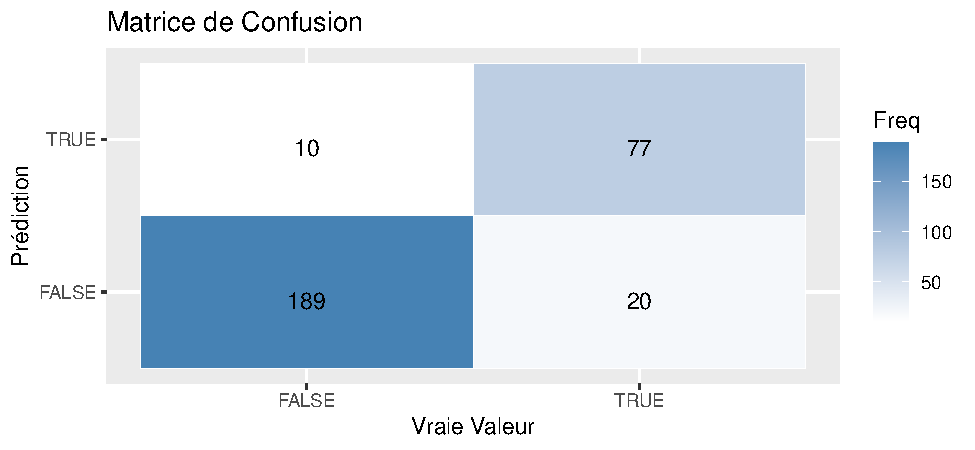
\includegraphics{Question-6_files/figure-latex/fig1-1.pdf} Nous obtenons
la figure \ref{fig:fig1}. Ce résultat a un taux de précision de :
0.8986486 . C'est très correct, car avec la LDA nous obtenions un taux
de 0.92 à peu près. Ainsi, en ne gardant que certaines variables, nous
obtenons un score plutôt proche. On en déduit que l'ammoniac, le
protoxyde d'azote, le type d'EPCI et l'année explique bien le
dépassement d'émission de méthane de 1000 t par an.

\end{document}
